\chapter{Interpretación y Resultados}
\label{ch:results}

En el presente capítulo se presentarán a detalle los resultados obtenidos por el módelo de pronóstico de demanda y maximización de ingresos. También se discutirá la forma en la que se deberán interpretar los resultados del mismo y así evitar sacar conclusiones erróneas o fuera de contexto.

\section*{Interpretación del modelo}

Como hemos mencionado en capítulos anteriores, el modelo propuesto se compone de dos módulos principales, el primero de ellos se encarga de pronósticar la demanda de cuartos noche para un día dado con cierto tiempo de anticipación, mientras que el segundo módulo toma esa información y cálcula los precios por habitación que maximizan el ingreso de la propiedad tomando en cuenta las restricciones definidas.

A continuación explicaremos detalladamente las salidas obtenidas en cada uno de los módulos definidos, la manera en que se deben interpretar esas salidas y los resultados obtenidos para el desempeño del modelo.

\subsection*{Pronóstico de Demanda}

El modelo de pronóstico de demanda toma como entrada las curvas de \emph{pickup} para una propiedad en específico, información de su ocupación histórica, lineas de tiempo de tarifa promedio, lineas de tiempo de tarifas publicas propias y de la competencia, etc. Al finalizar el procesamiento de la información se obtiene una matriz que contiene, entre otras variables, el parámetro $\beta_0$ y $\beta_1$ con el que se puede reconstruír la curva de pickup para un día futuro. De esta manera podemos obtener una buena aproximación de los cuartos que serán vendidos en cierto día y con qué velocidad se realizará esta venta.

A continuación se presenta un extracto de los resultados obtenidos por el modelo de pronóstico de demanda:

\begin{verbatim}
##   hotel        dia  AAbeta0       AAbeta1 AAvariacion
## 1 CEINS 2018-01-01 2.335294 -2.489863e-06   0.1884625
## 2 CEINS 2018-01-02 2.984073 -2.818019e-06   0.1321997
## 3 CEINS 2018-01-03 3.301841 -3.535574e-06   0.3262416
## 4 CEINS 2018-01-04 3.782523 -2.295688e-06   0.1744051
## 5 CEINS 2018-01-05 3.761697 -1.089675e-06   0.0925871
## 6 CEINS 2018-01-06 3.140137 -2.292639e-06   0.1887511
##       tdc       PO       PT    diasem  mes eventos1 eventos
## 1 19.7354 0.840382 0.872720     lunes ene.        0       0
## 2 19.7354 1.096970 1.025310    martes ene.        0       0
## 3 19.6629 0.927171 0.992081 miércoles ene.        0       0
## 4 19.4899 1.045640 1.024860    jueves ene.        0       0
## 5 19.3717 0.927771 0.953648   viernes ene.        0       0
## 6 19.2427 1.334990 0.908828    sábado ene.        0       0
##   pred.beta0  pred.beta1
## 1   3.159533 -0.12278602
## 2   3.916035 -0.11603131
## 3   3.874017 -0.10891126
## 4   4.159721 -0.10283409
## 5   3.698266 -0.08467446
## 6   3.771660 -0.09371103
\end{verbatim}

Para poder reconstruír la curva de \emph{pickup} pronosticada se debe tomar los parámetros \emph{pred.beta0} y \emph{pred.beta1} para evaluar la siguiente expresión: $$E[y|x]=e^{\beta_0 + \beta_1x}$$

Dónde:
\begin{itemize}[noitemsep]
\item $E[y|x]$ = El valor esperado de cuartos noches para un día en específico dado $x$ días de antelación
\item $\beta_0$ = pred.beta0
\item $\beta_1$ = pred.beta1
\item $x$ = días de antelación
\end{itemize}

Evaluando esta expresión en distintas fechas obtenemos las siguientes curvas de pronóstico de ocupación:

\definecolor{shadecolor}{rgb}{0.969, 0.969, 0.969}\color{fgcolor}
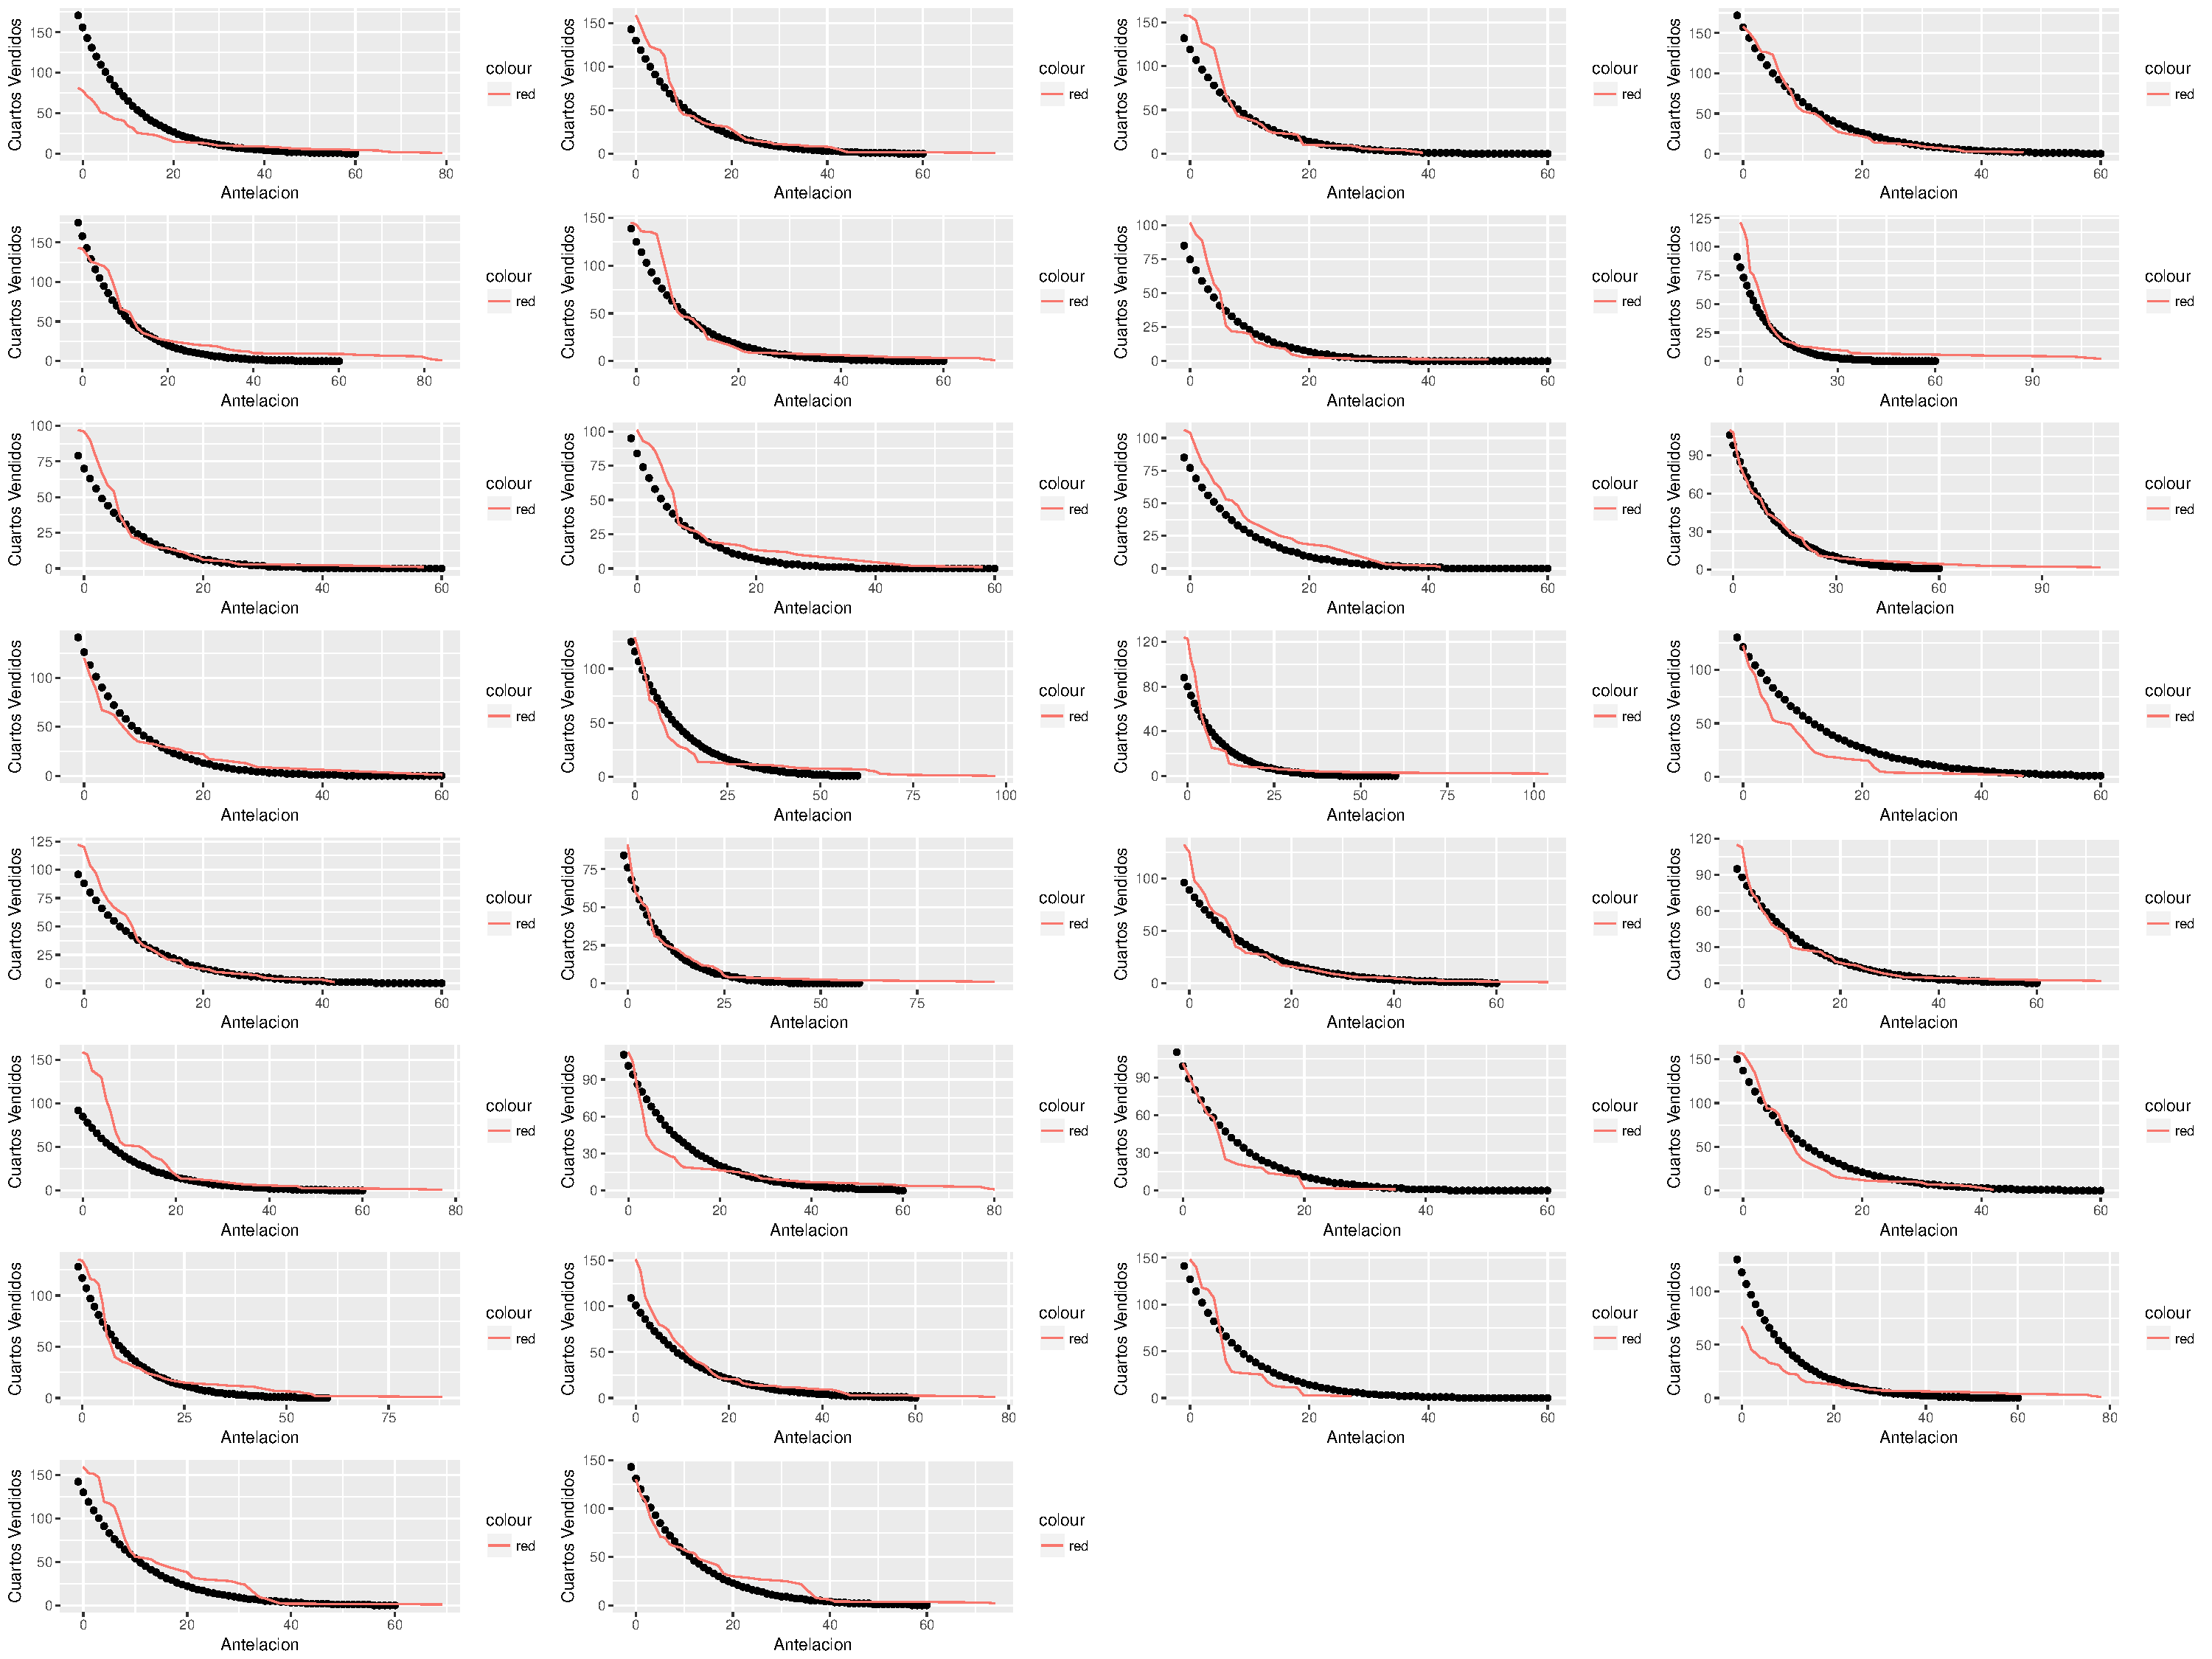
\includegraphics[width=\maxwidth]{Figures/ValidacionModelo-1} 

Podemos observar que la curva pronosticada tiene un buen ajuste sobre la curva real en la mayoría de los casos.

Para realizar la validación del modelo se dividió el data set en dos partes, la primera parte se utilizó para el entrenamiento del modelo y la segunda parte para la validación del mismo, de esta forma se pudo comparar el pronóstico de demanda arrojado por el modelo contra la demanda real de la propiedad en 220 días para el año 2018.

Para evaluar el desempeño del modelo se utilizó la medida \emph{MAPE} definida como: $$MAPE=\frac{1}{n}\sum_{t=1}^{n}|\frac{y_t-h_t}{y_t}|$$

Dónde:
\begin{itemize}[noitemsep]
  \item n = Número de puntos ajustados
  \item $y_t$ = Cuartos noche vendidos en el tiempo $t$
  \item $h_t$ = Venta de cuartos noche pronósticada en el tiempo $t$
\end{itemize}


El \emph{MAPE} observado durante la validación del modelo fue de 17.67\% que de acuerdo con la investigación realizada en el capítulo dos está dentro de los parámetros aceptables.


\subsection*{Modelo de maximización de ingresos}

El modelo de recomendaciones de precio toma como entrada la demanda pronósticada por el módelo de pronóstico de demanda. A partir de ahi, se define un problema de maximización sujeto a restricciones y se arroja una matriz que contiene los precios para un tipo de cuarto dependiendo del inventario disponible dentro de la propidad.

A continuación se muestra un extracto del resultado:

\begin{verbatim}
##            day       40       80       120       159
## 137 2018-05-17 1616.650 1374.773 1122.4972  975.1633
## 77  2018-03-18 1701.113 1675.709 1368.2105 1188.6253
## 52  2018-02-21 1666.334 1529.706 1248.9996 1085.0615
## 16  2018-01-16 1647.043 1463.557 1194.9895 1038.1406
## 24  2018-01-24 1702.217 1681.071 1372.5888 1192.4289
## 93  2018-04-03 1703.315 1686.416 1376.9532 1196.2205
## 78  2018-03-19 1621.479 1387.804 1133.1372  984.4067
## 167 2018-06-16 1498.239 1138.420  929.5160  807.5119
## 139 2018-05-19 1527.223 1184.905  967.4709  840.4850
## 174 2018-06-23 1518.070 1169.615  954.9869  829.6396
\end{verbatim}

La manera en la que se debe interpretar esta matriz es la siguiente: Para el día 17 de mayo de 2018, las habitaciones sencillas de este hotel deben de tener un precio de 975.16 MXN si el inventario disponible esta entre 121 y 159 habitaciones disponibles. Si se tienen entre 81 y 120 habitaciones disponibles, el precio debe de ser de 1122.49 MXN y así sucesivamente. De esta manera podemos asignar un lote de habitaciones a diferentes rangos de precios siendo las últimas habitaciones disponibles las que tengan el precio más alto.


A continuación se presenta una gráfica con los resultados obtenidos por el modelo de maximización de ingresos:

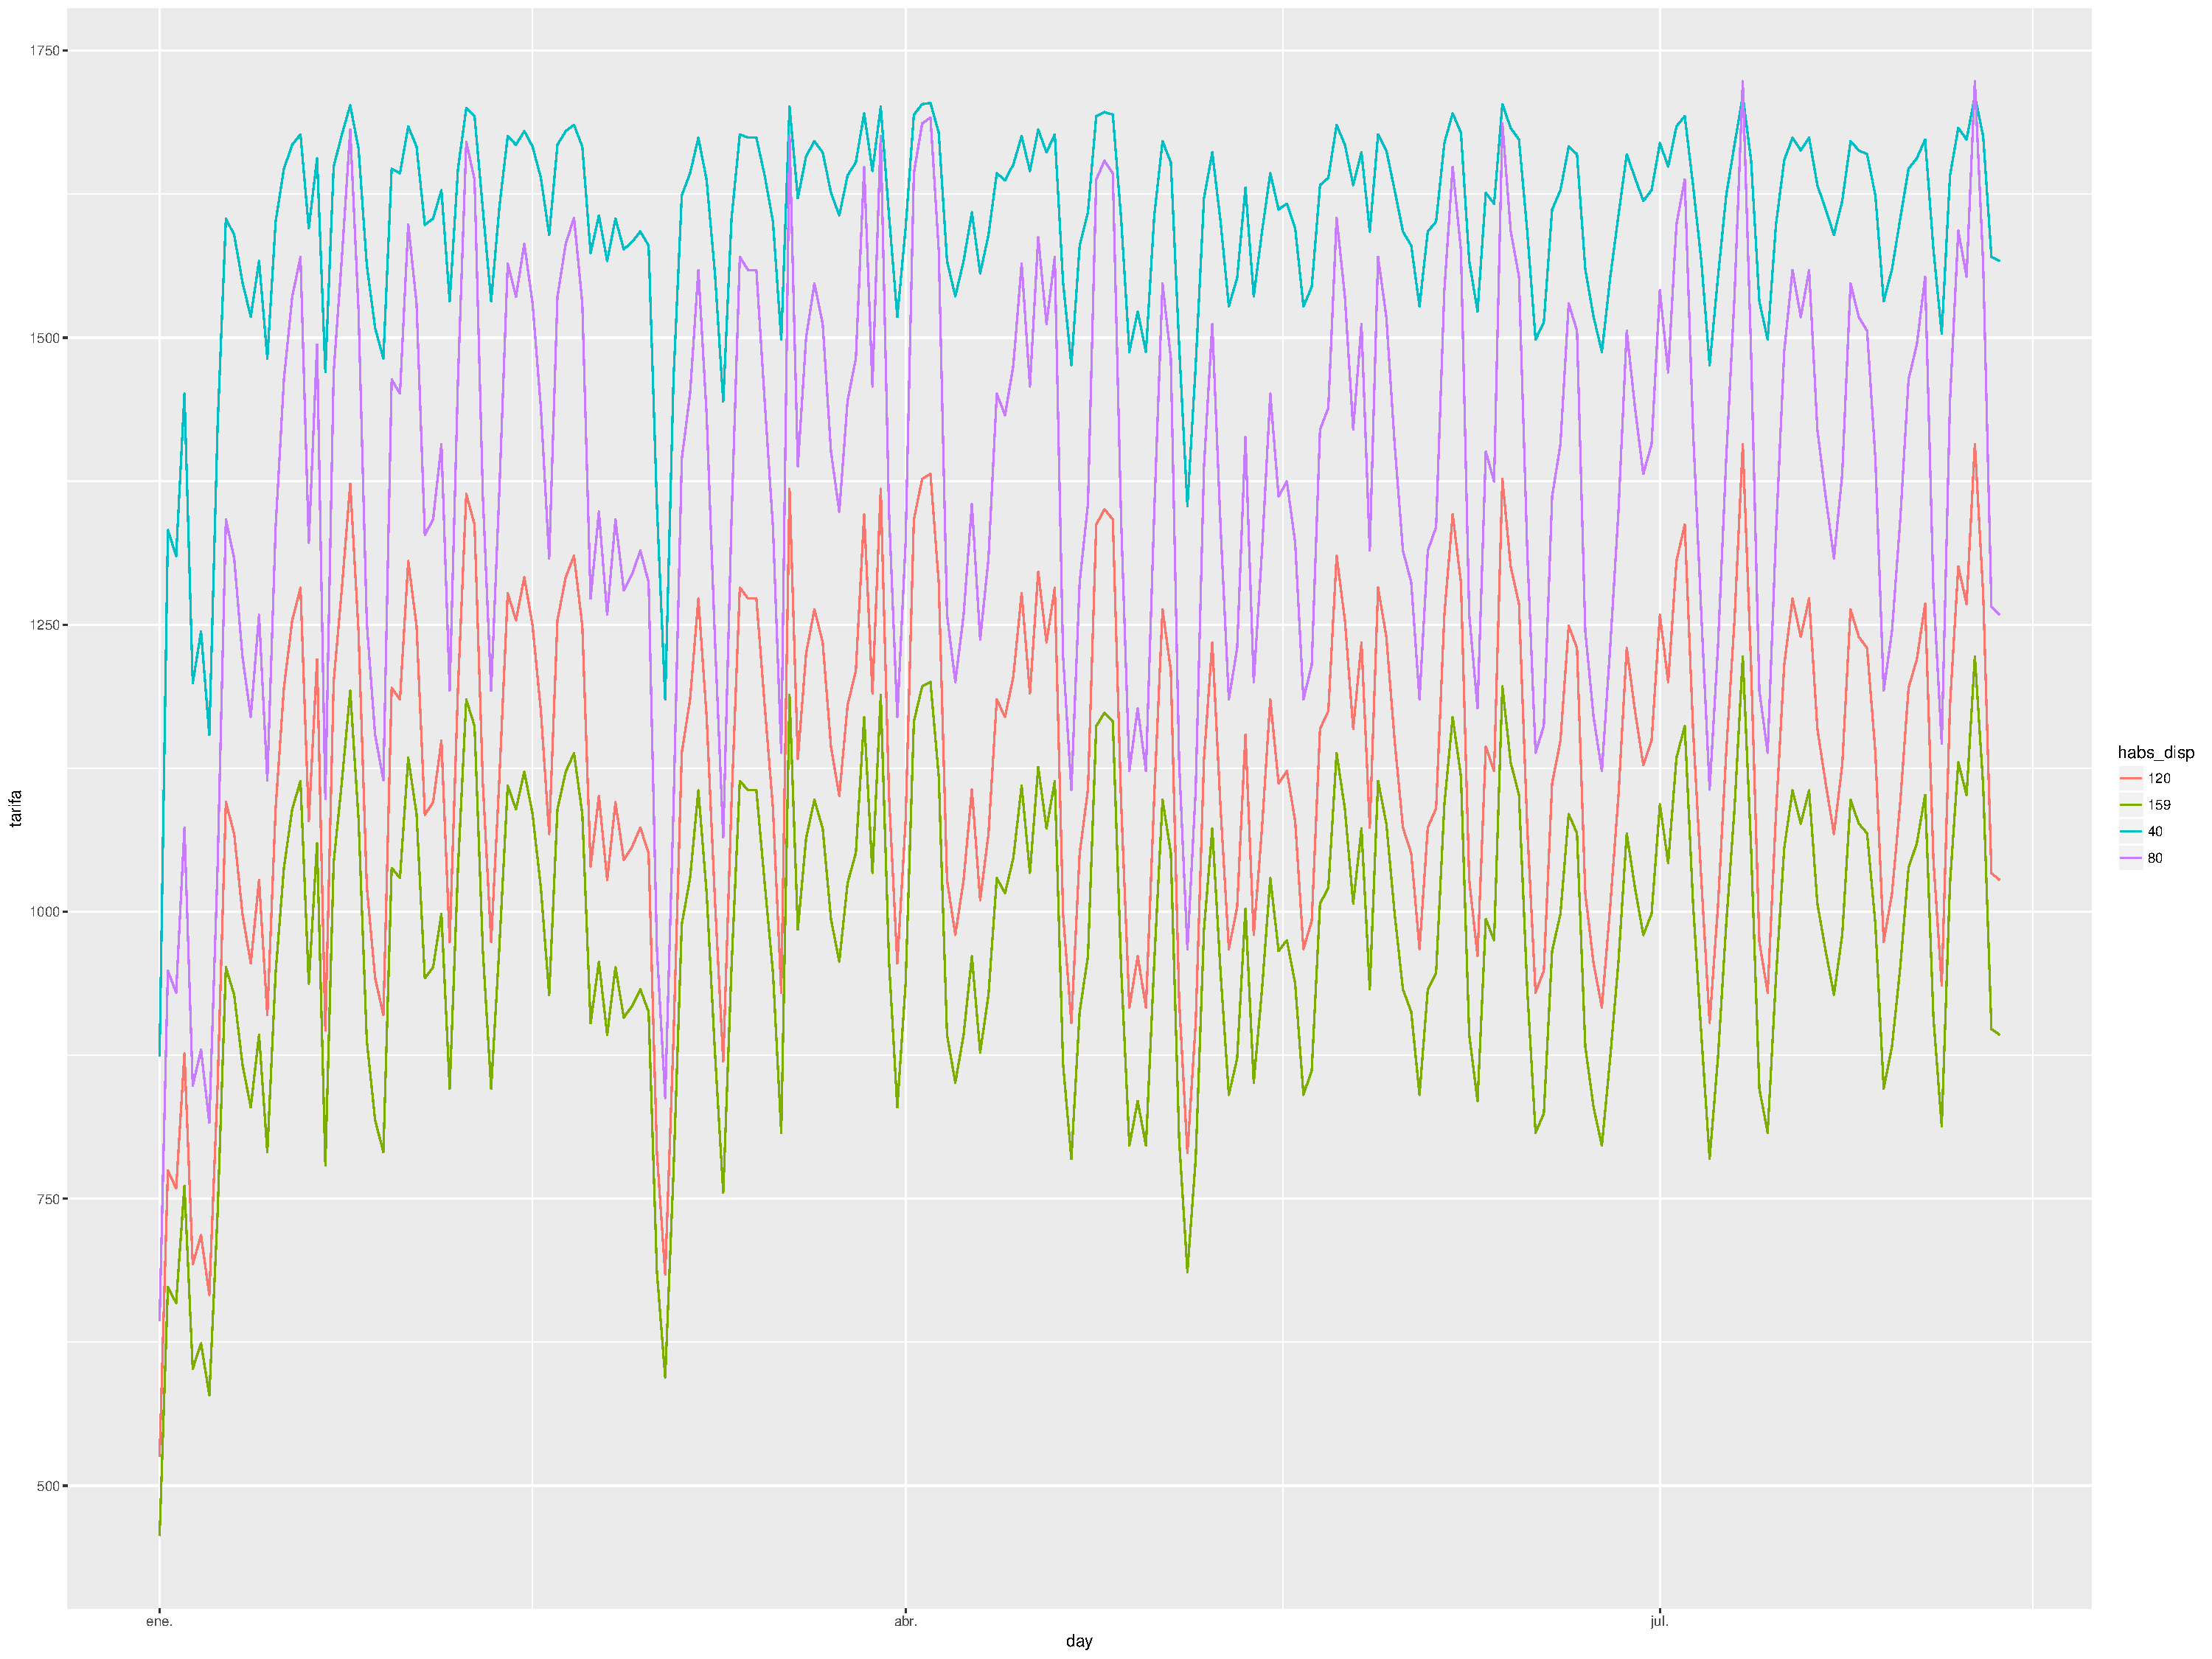
\includegraphics[width=\maxwidth]{figures/Pricing_graph-1} 

Para medir el desempeño del modelo de maximización de ingresos, se tomaron los resultados y se calcularon las tarifas promedio a partir de los datos obtenidos y se compararon contra las tarifas promedio reportadas por la propiedad para el año 2018.

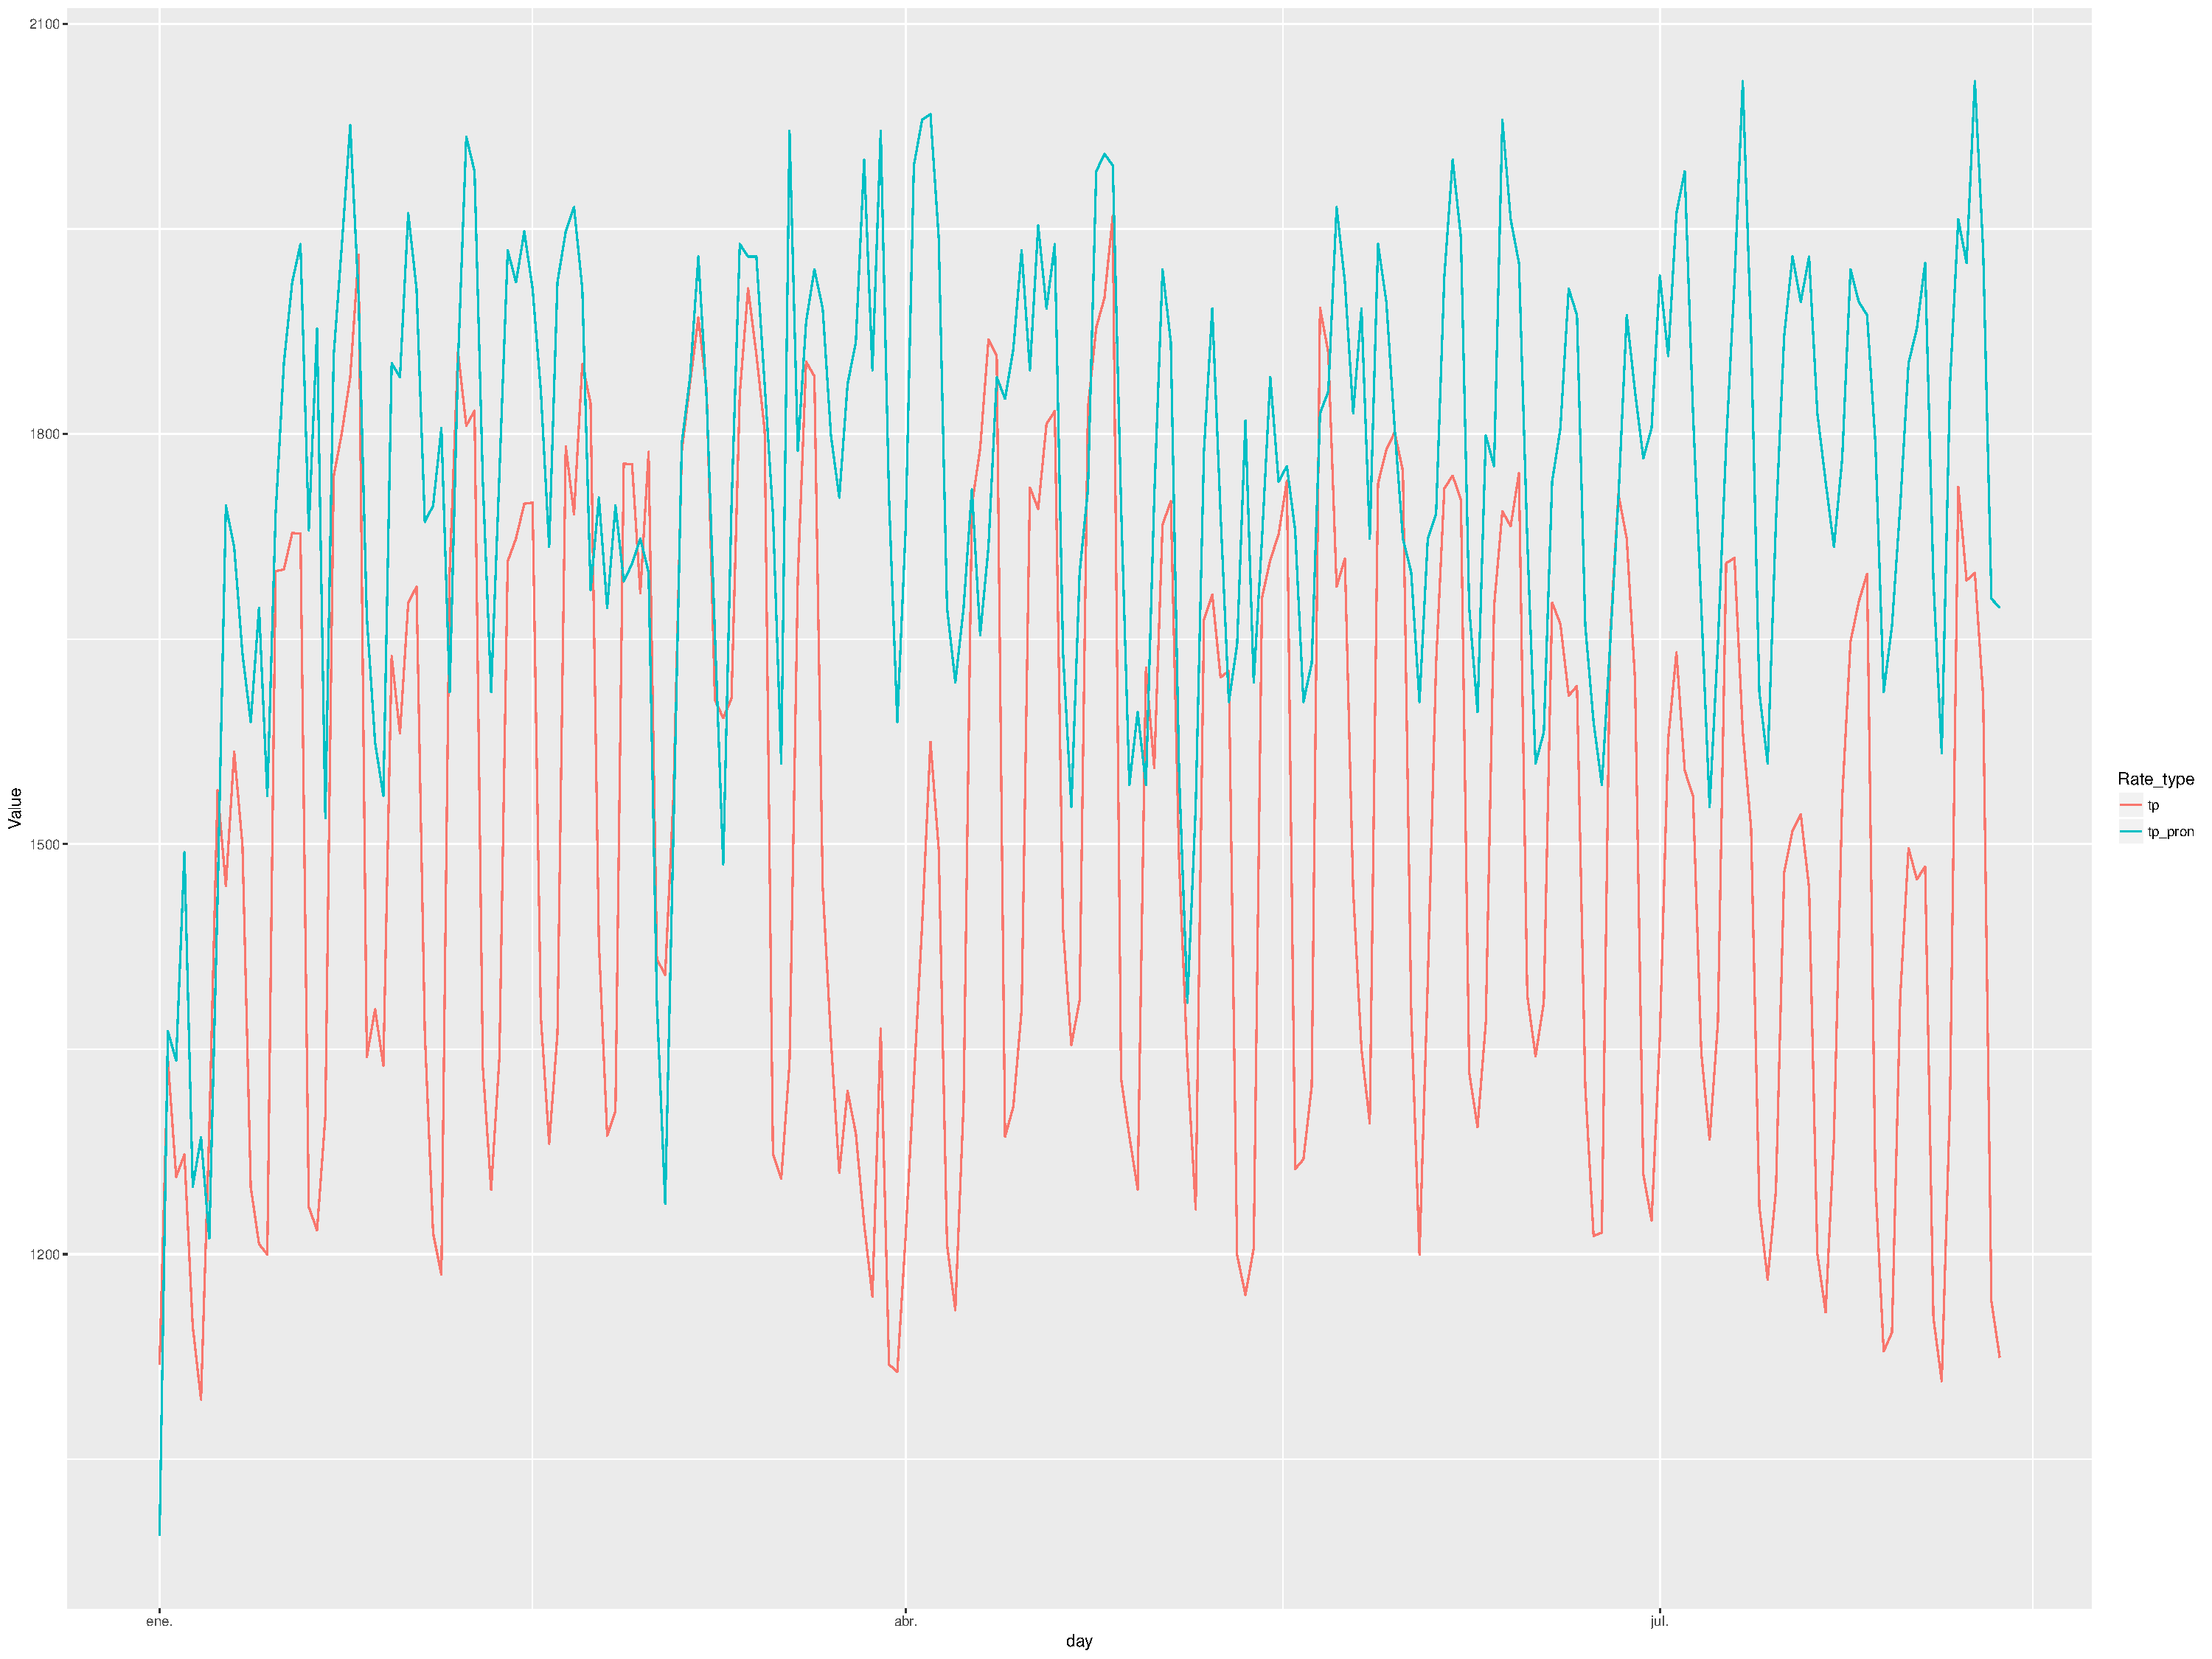
\includegraphics[width=\maxwidth]{figures/Pricing-1} 

Si obtenemos la diferencia de tarifas promedio, notamos que si se utilizara el resultado del modelo de optimización tendríamos un aumento en los ingresos de aproximadamente 57555.70 MXN. Sin embargo, para poder validar este resultado se propone implementar este modelo dentro de la propiedad y comprobar sus resultados en la operación.




